\chapter{Models, Simulations and Findings}

%Check for mail with subject "Energy diagrams for hexagonal cell"

\section{Deployable Origami Tubes}
Two types of triangulated Origami tubes were developed and were tested for deployability. In accordance with the idea of energy profile based on the sum of two angles of the triangular units of the tubes easy-deploy-easy-collapse and hard-deploy-hard-collapse tubes were developed\cite{Zha}. 

The cylindrical tube is generated by joining two edges of the sheet show in the Fig~\ref{fig:AlphaBeta}. For the angles shown in Fig~\ref{fig:AlphaBeta}, if $\alpha + \beta < 90^{\circ}$ the tube is of the easy-deploy-easy-collapse (Fig~\ref{fig:EDEC}) type and if the sum is greater than $90^{\circ}$ i.e $\alpha + \beta > 90^{\circ}$ the mechanism is of hard-deploy-hard-collapse type(Fig~\ref{fig:HDHC}). It was observed from analysis of numerical model that for the hard-deploy-hard-collapse model ($\alpha = 50^{\circ}, \beta = 50^{\circ}$), the strain in equivalent bar hinge model would be of the order 20\% and hence the collapse is not possible in normal paper model. Also the hard-deploy-hard-collapse model carried significant lode before the paper model underwent local buckling at its creases.
\begin{figure}[htbp]
\centering
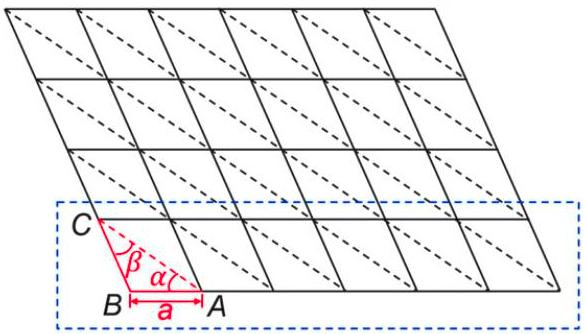
\includegraphics[width=0.6\linewidth]{introduction/fig/AlphaBeta.jpg}
\caption{Crease Pattern For Cylindrical Tube}
\label{fig:AlphaBeta}
\end{figure}

\begin{figure}
\centering
\begin{minipage}{.5\textwidth}
  \centering
  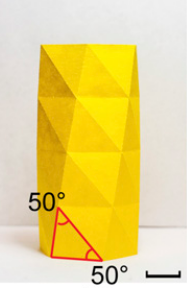
\includegraphics[width=.4\linewidth]{introduction/fig/HardDeploy.png}
  \captionof{figure}{Hard-Deploy-Hard-Collapse}
  \label{fig:EDEC}
\end{minipage}%
\begin{minipage}{.5\textwidth}
  \centering
  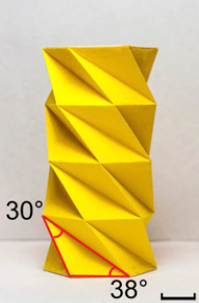
\includegraphics[width=.4\linewidth]{introduction/fig/EasyDeploy.png}
  \captionof{figure}{Easy-Deploy-Easy-Collapse}
  \label{fig:HDHC}
\end{minipage}
\end{figure}


\section{Energy Profiles}
The simulated energy profiles for the origami tubes are shown in the Fig~\ref{fig:EnergyProfile}. The simulation was performed for the equivalent bar hinge model.
\begin{figure}[htbp]
\centering
	\subfigure[Easy-Collapse-Easy-deploy energy profile ]{
	\centering
		\label{fig:ECEDEP}
        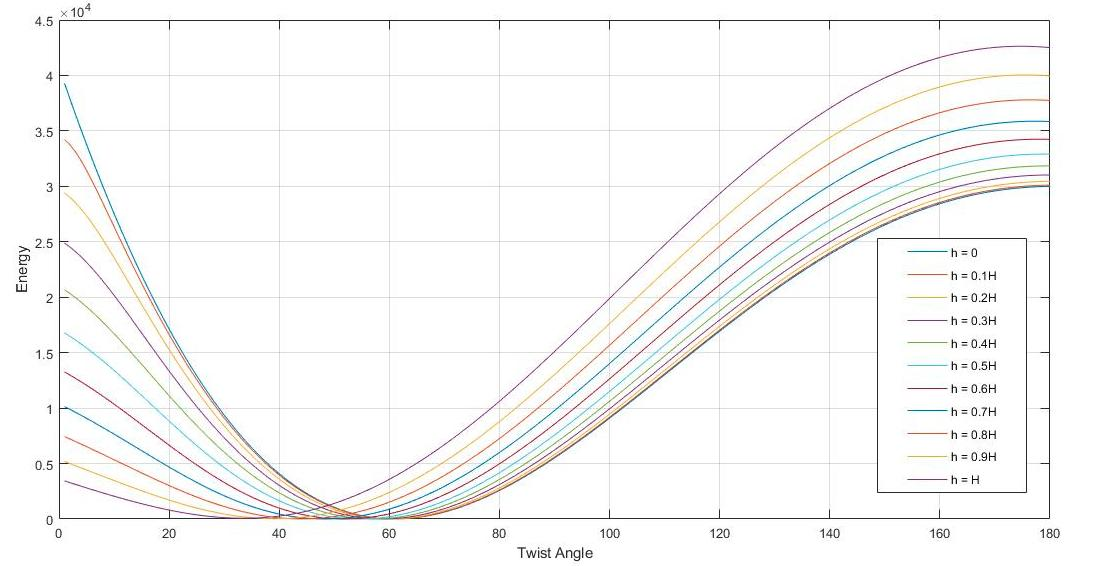
\includegraphics[width=1\linewidth]{introduction/fig/EDEC.jpg}}
	\subfigure[Hard-Collapse-Hard-deploy energy profile]{
	\centering
		\label{fig:HCHDEP}
		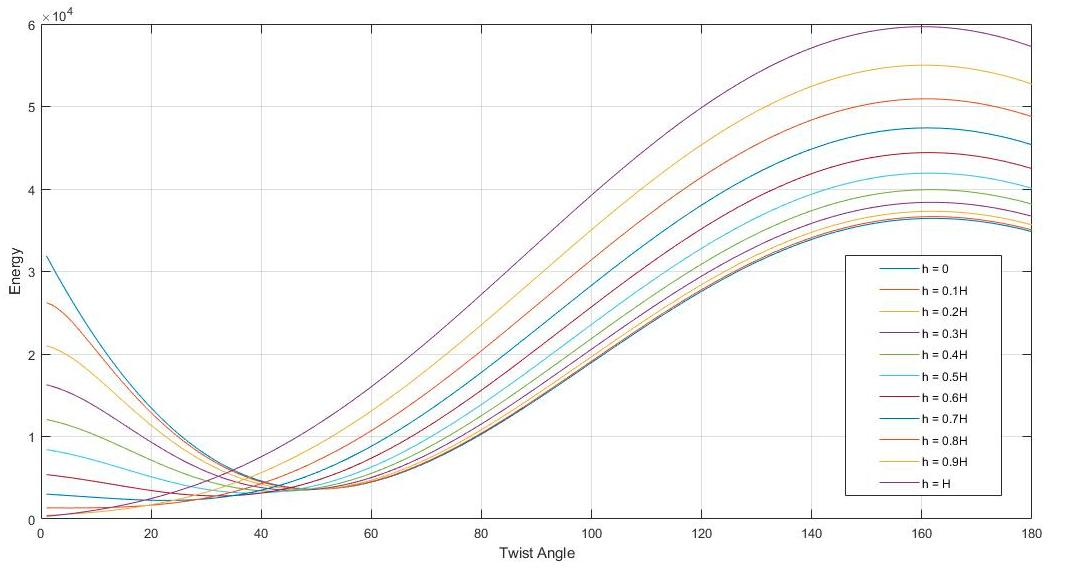
\includegraphics[width=1\linewidth]{introduction/fig/HDHC.jpg}}
	\caption{Energy Profiles}
	\label{fig:EnergyProfile}
\end{figure}

As it can be seen from the energy profile obtained by computing energy in the structure at various stages of deployment, the easy-deploy-easy-collapse structure presents negligible energy barrier as opposed to the hard-deploy-hard-collapse structure in which significant energy barrier is present for process of deployment as well as collapse. 

Using metamaterials, a structure which presents no energy barrier during deployment but exhibits resistance to collapse can be developed. This will provide the reliability to the deployable structure without being dependent on locking mechanisms for its stability.

\section{Lattices}
The current work is directed towards developing a Julia program which can generate lattices and predict the behavior of lattice using simple spring ball models. Currently the effort is directed toward developing a program which can create finite lattices with provided boundary conditions. Small displacements are provided in direction normal to lattice to induce out of plane curvatures. A sample rectangular lattice generated using the Julia program is presented in the Fig~\ref{fig:RectLattice}.
\begin{figure}[htbp]
    \centering
    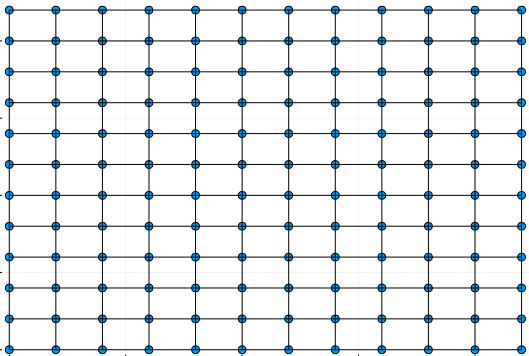
\includegraphics[width = 1\linewidth]{introduction/fig/lattice.png}
    \caption{Rectangular lattice}
    \label{fig:RectLattice}
\end{figure}{}